\chapter{Implementation}

\section{AWS IoT Core}

As part of this project, we chose the \ac{iot} Framework \ac{aws} \ac{iot} Core. 
The core function of this IoT framework is the secure and reliable communication between IoT devices, which is made possible using standard \ac{iot} protocols such as \ac{mqtt}, \ac{https} or WebSockets. 
In order to enable communication between \ac{aws} \ac{iot} Core and our smart factory simulator, a virtual preprenation of the \ac{iot} devices, so-called things, first had to be defined in the \ac{aws} \ac{iot} Framework. 

\begin{figure}[H]
	\centering
	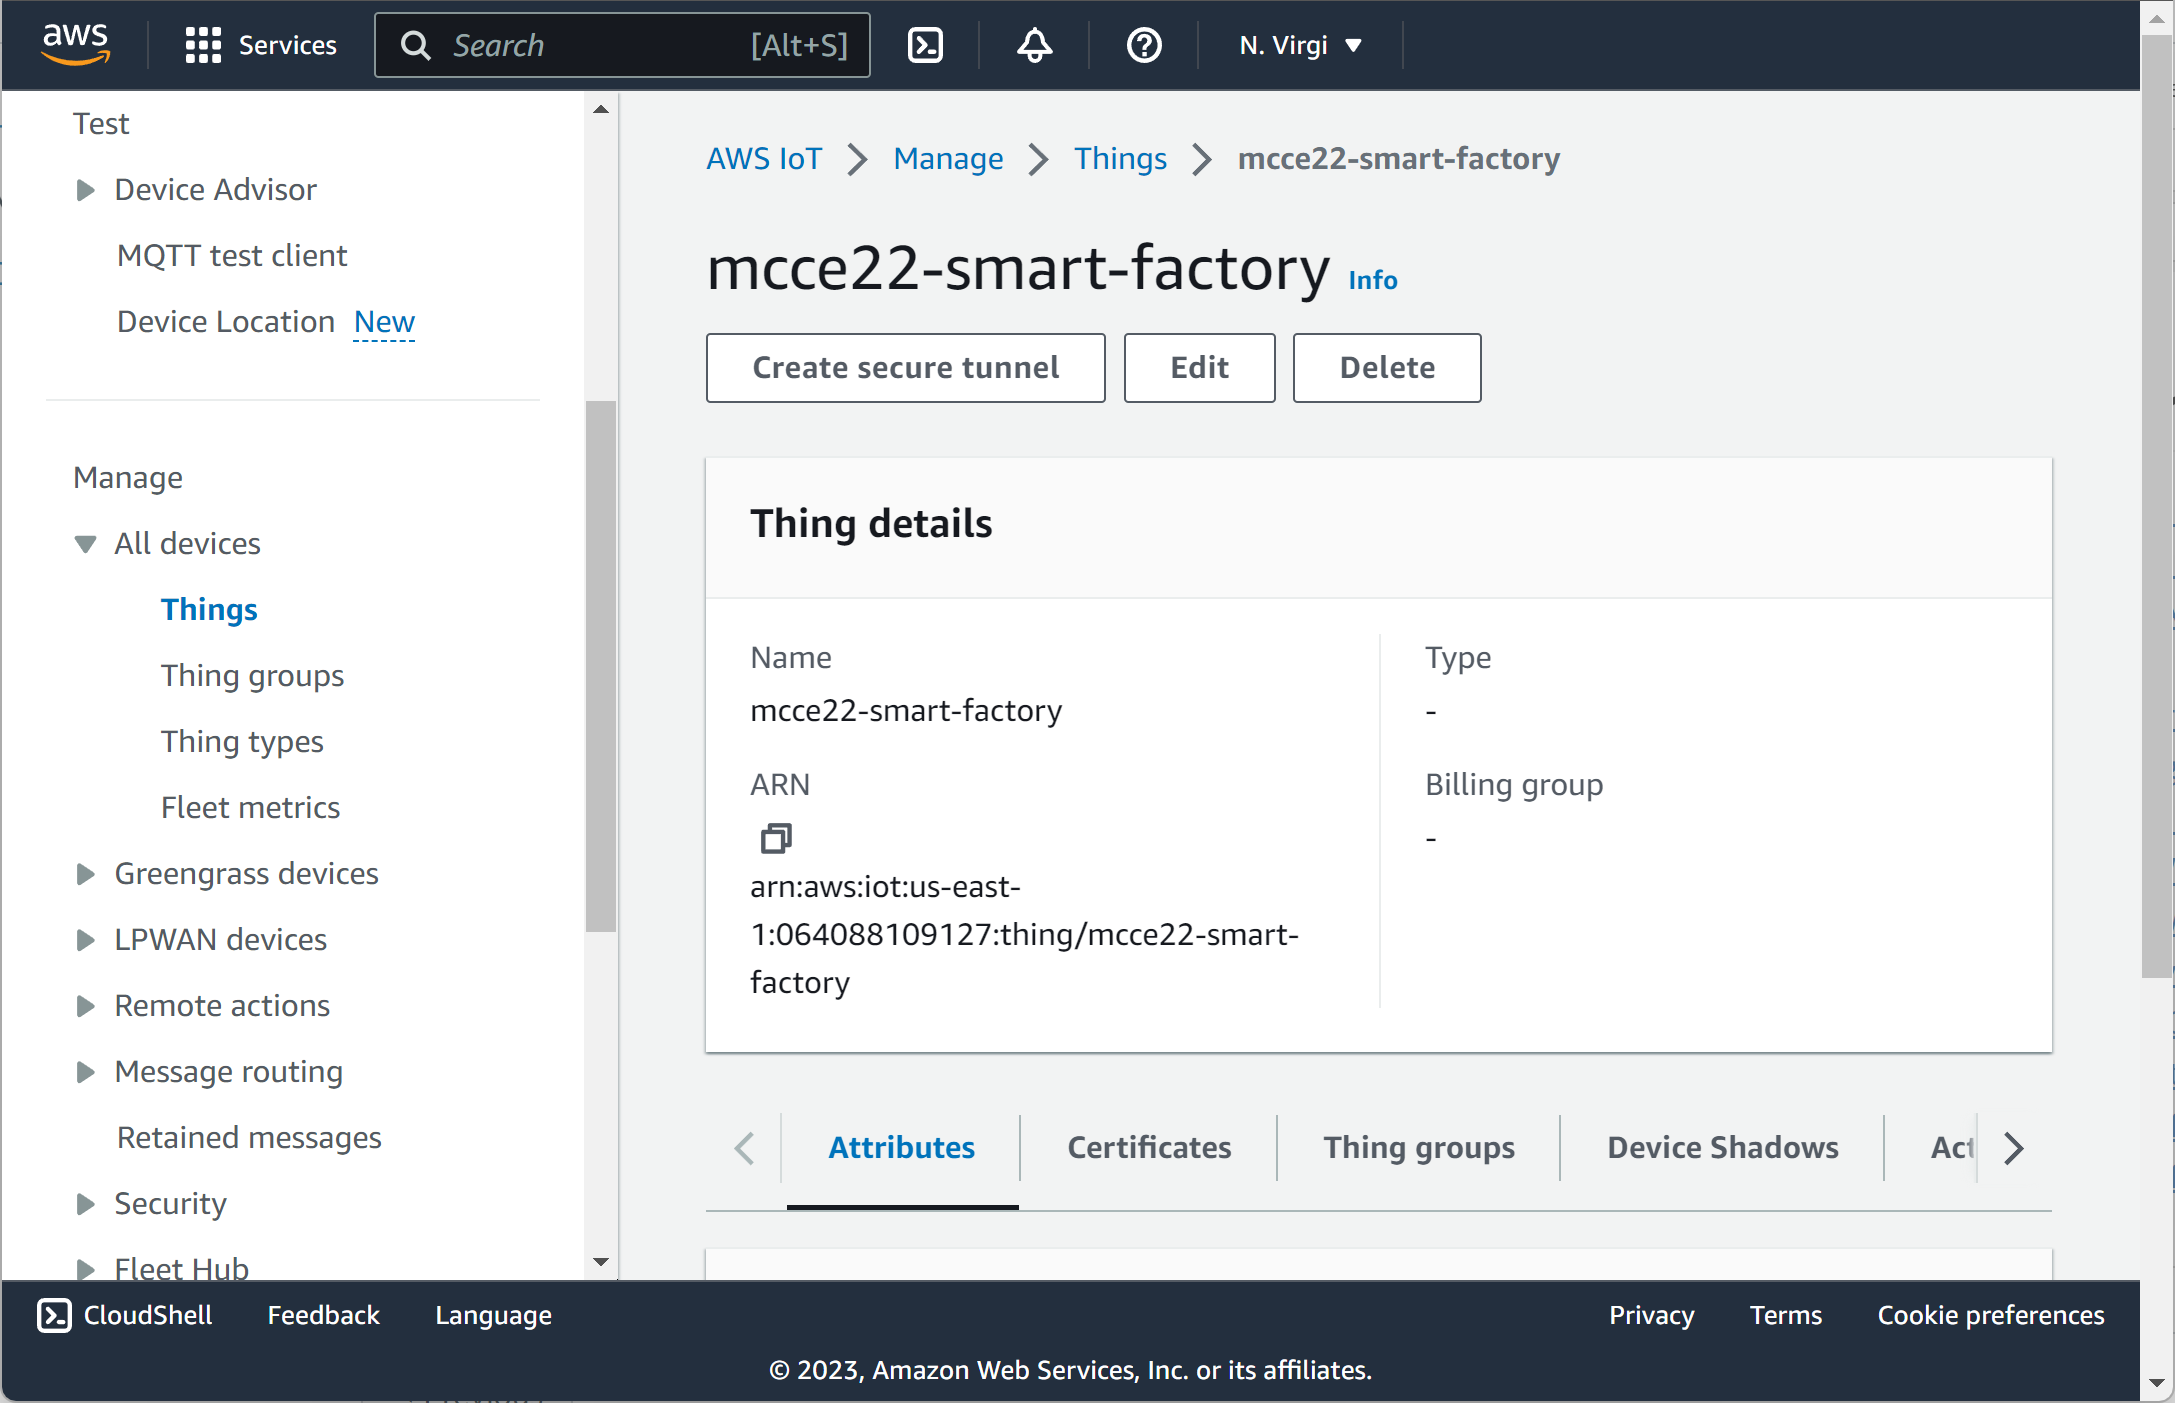
\includegraphics[width=15cm]{images/smart_factory_thing.png}
	\caption{\ac{aws} \ac{iot} Core Thing}    
	\label{fig:SmartFactoryThing}
\end{figure}

Figure \ref{fig:SmartFactoryThing} shows the configuration of such a virtual representation of an \ac{iot} device in \ac{aws} \ac{iot} Core. 
This definition of virtual things is an essential part of IoT Core security system, since a combination of private and public certificate pairs is generated for each defined thing.
These certificates are then required for secure communication with the \ac{aws} \ac{iot} Core Message Broker. 
In the case of our Smart Factory Simulator there is only one client that communicates with the message broker of \ac{aws} \ac{iot} Core and therefore only one virtual thing has been created. 
In a real world scenario, in which each sensor, actuator or button of the smart factory is  represented by its own \ac{iot} device, there would be one thing definition for each physical device.

\section{IoT Simulator}
Initially it was planned to simulate the sensors, actuators and buttons as well as the required control loops using the \ac{aws} \ac{iot} Simulator. 
\ac{aws} \ac{iot} Simulator is a collection of different AWS tools that allow users to test and simulate the behavior of \ac{iot} devices and their interactions with the \ac{aws} \ac{iot} platform without requiring any physical hardware. 
The required tools are provided directly in your own AWS account using infrastructure as code.
Unfortunately, some tools and features required by the \ac{aws} \ac{iot} Simulator were not available in the FH Burgenland \ac{aws} LAB environment, which is why an alternative approach for simulating the Smart Factory \ac{iot} devices had to be chosen.

In order to still be able to show the interaction of the individual sensors, actuators and buttons of the Smart Factory, a small simulator was implemented for the visualization and the implementation of the required control loops. 
Figure \ref{fig:SmartFactorySimulator} shows the Smart Factory simulator and highlighted the implemented use cases.

\begin{figure}[H]
	\centering
	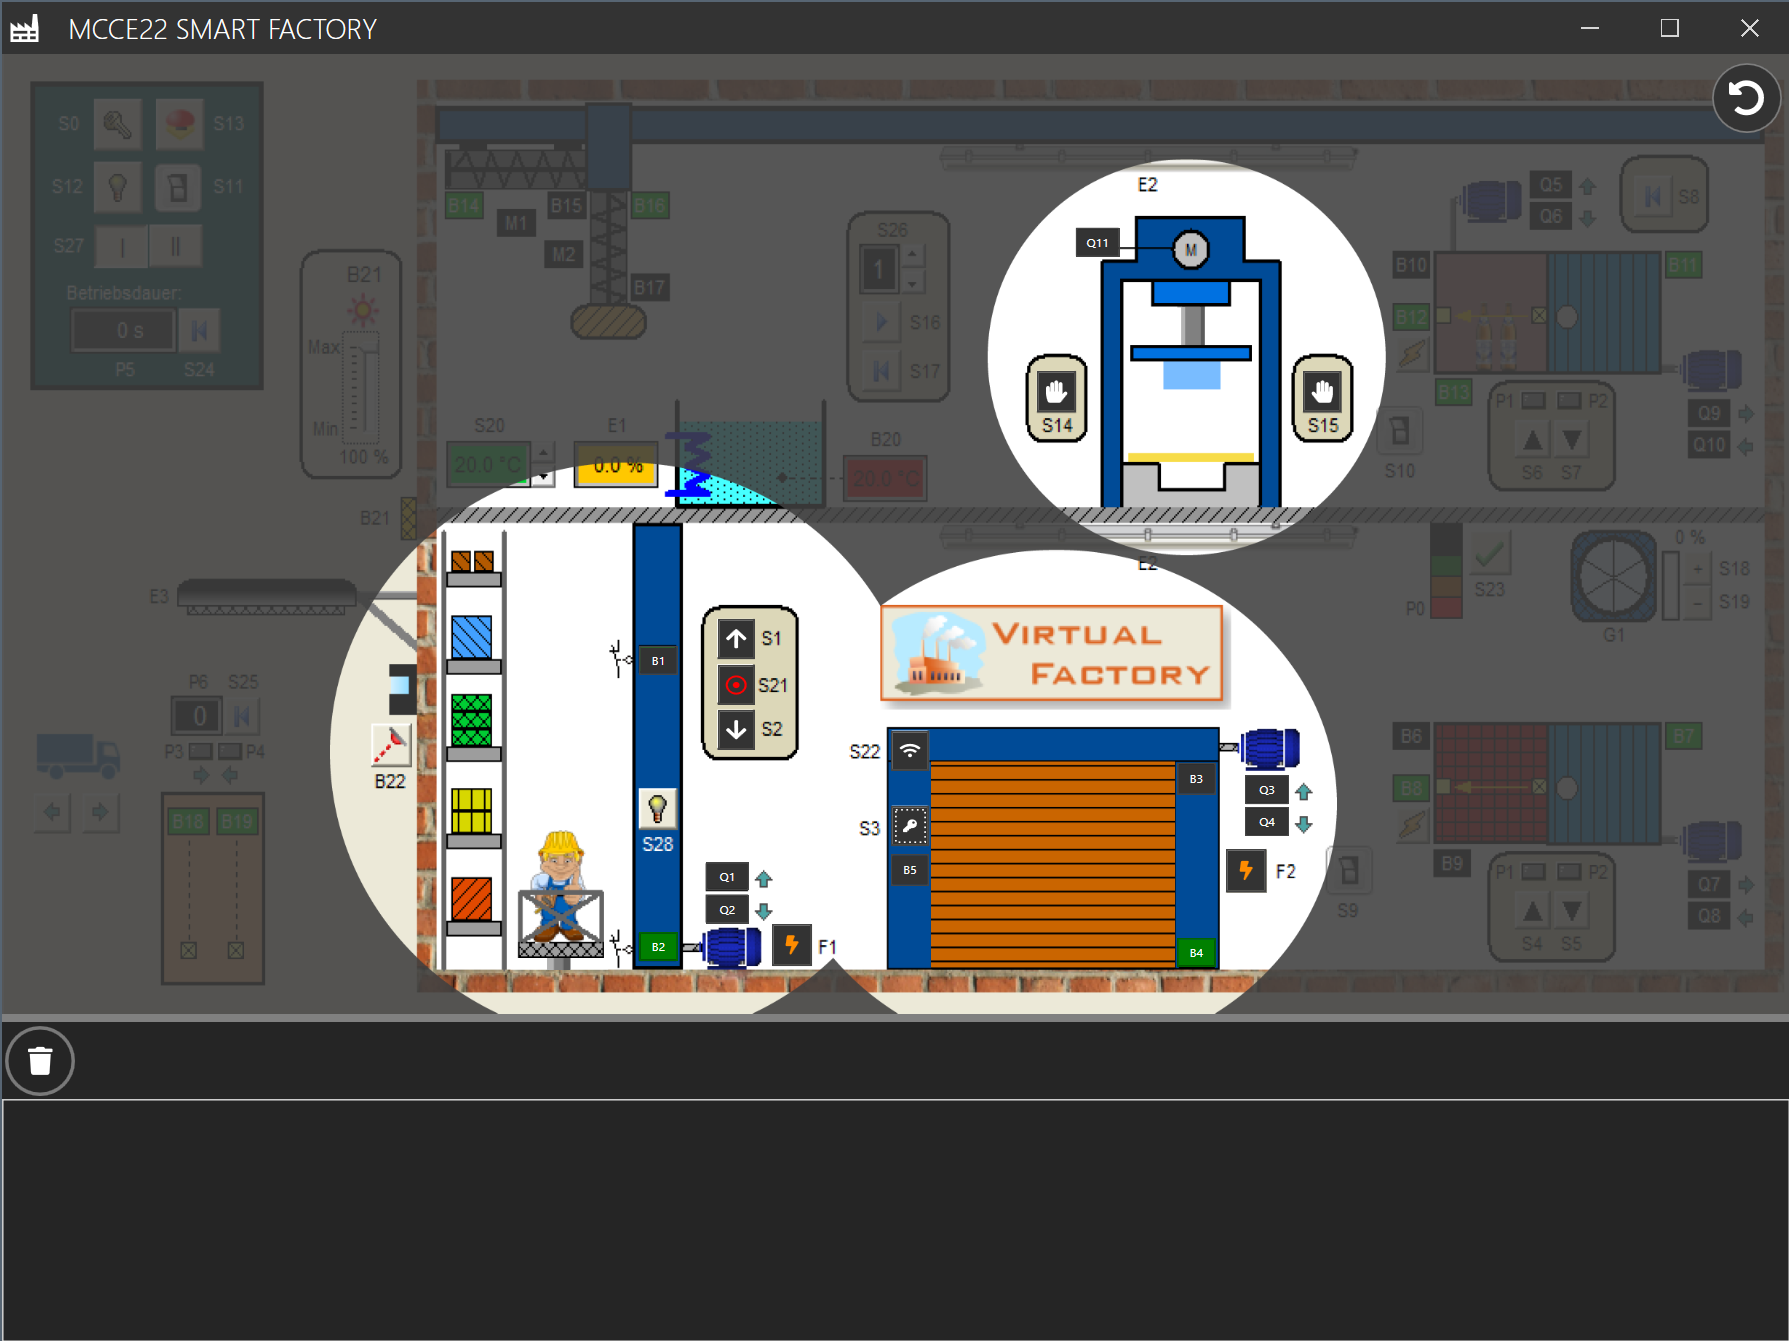
\includegraphics[width=15cm]{images/smart_factory_simulator.png}
	\caption{Smart Factory Simulator}    
	\label{fig:SmartFactorySimulator}
\end{figure}

\textbf{.NET Core}

.NET Core is a free, open-source, cross-platform framework for building modern applications. 
It is a successor to the .NET Framework and provides a set of tools, libraries and runtime environments for building applications for Windows, Linux and macOS operating systems.

\textbf{\ac{wpf}}

\ac{wpf} is a graphics framework of the .NET Framework from Microsoft. 
It provides a powerful set of features for creating visually appealing and interactive user interfaces. \ac{wpf} also includes a rich set of controls that can be used to create common user interface elements such as buttons, text boxes, and menus. 
In addition, WPF offers the possibility to define animations and transitions. 
These animations cabalitites where used to realize the moving transitions of the different parts in the Smart Factory simulator.

\textbf{MaaApps.Metro}

MahApps.Metro is an open-source library that can be used to create modern, stylish and functional Windows desktop applications. 
It's built on Microsoft's \ac{wpf} framework and offers a set of controls, styles, and templates that make it easy to create professional-looking applications.

\textbf{MQTTnet}

MQTTnet is a powerful and open source C\# library to simplify MQTT-based communication. 
In Smart Factory simulator, this library was used to establish the communicate with \ac{aws} \ac{iot} Core.

In order to implement the function of the sensors, actuators and buttons as realistically as possible, a separate class was implemented for each of these components. 
This encapsulation allowed the behavior of each component to be implemented separately and independently. 
All communication between these classes was done exclusively by exchanging MQTT messages using AWS IoT Core. 
Each implementation of a sensor, actuator or button only subscribes to the MQTT topics that is required for its function or control loop. Figure \ref{fig:FlowChartS3} shows the flowchart of the control loops for S3 that were used to automate the factory door. The following \ac{mqtt} topics were defined for the implementation of the 4 use cases:

\begin{itemize}
	\item mcce22-smart-factory/door
	\item mcce22-smart-factory/lifter
	\item mcce22-smart-factory/press
	\item mcce22-smart-factory/light
\end{itemize}

\begin{figure}[H]
	\centering
	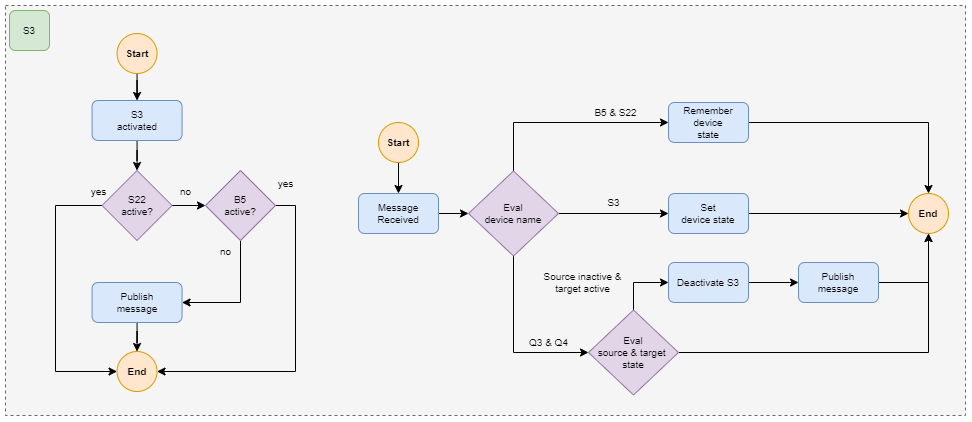
\includegraphics[width=15cm]{images/flowchart_s3.png}
	\caption{S3 Control Loops}    
	\label{fig:FlowChartS3}
\end{figure}

Since S3 is a button, there are two possible control loops. The first describes manually triggering the button while loop two is started by receiving a message from AWS IoT Core. Figure \ref{fig:FlowChartQ3}  shows the control loop for the factory gate motor Q3 and how it is controlled by receiving messages from AWS IoT Core triggered from other sensors or buttons.

\begin{figure}[H]
	\centering
	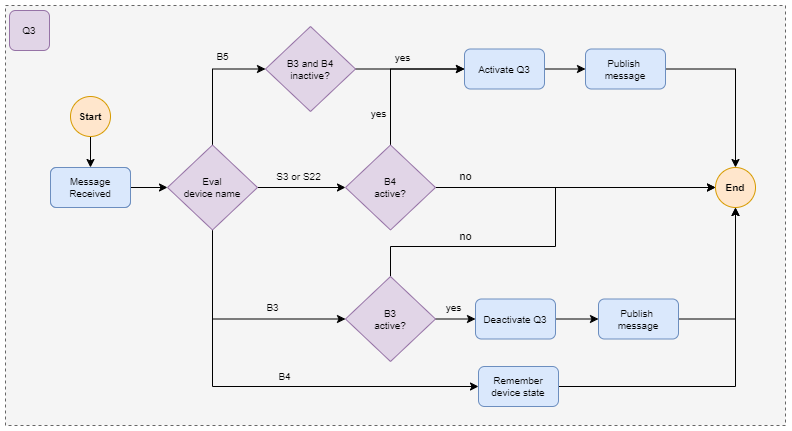
\includegraphics[width=13cm]{images/flowchart_q3.png}
	\caption{Q3 Control Loop}    
	\label{fig:FlowChartQ3}
\end{figure}
